\documentclass{article}
\usepackage{amsmath}
\usepackage{tikz}
\usetikzlibrary{shapes.geometric}

\begin{document}

\begin{figure}[h]
    \centering
    \begin{tikzpicture}[scale=0.5]
        % Draw the grid
        \draw[help lines] (0,0) grid (8,8);
        
        % Draw the red shaded areas
        \fill[red!20] (0,0) rectangle (2,4);
        \fill[red!20] (6,0) rectangle (8,4);
        \fill[red!20] (0,4) rectangle (2,8);
        \fill[red!20] (6,4) rectangle (8,8);
        
        % Draw the blue rectangles
        \foreach \x in {3,4} {
            \foreach \y in {1,2,3} {
                \node[draw, fill=blue!20, minimum width=0.5cm, minimum height=0.5cm] at (\x,\y) {};
            }
        }
        \foreach \x in {5,6} {
            \foreach \y in {1,2,3} {
                \node[draw, fill=blue!20, minimum width=0.5cm, minimum height=0.5cm] at (\x,\y) {};
            }
        }
        
        % Draw the blue lines
        \draw[blue, thick] (3.5,1) -- (3.5,3);
        \draw[blue, thick] (4.5,1) -- (4.5,3);
        \draw[blue, thick] (5.5,1) -- (5.5,3);
        \draw[blue, thick] (6.5,1) -- (6.5,3);
        
        % Draw the red triangles
        \foreach \x in {1,2} {
            \foreach \y in {1,2,3} {
                \node[draw, fill=red!50, minimum width=0.5cm, minimum height=0.5cm, shape=isosceles triangle, rotate=90] at (\x,\y) {};
            }
        }
        \foreach \x in {7,8} {
            \foreach \y in {1,2,3} {
                \node[draw, fill=red!50, minimum width=0.5cm, minimum height=0.5cm, shape=isosceles triangle, rotate=90] at (\x,\y) {};
            }
        }
        
        % Draw the red triangles
        \foreach \x in {1,2} {
            \foreach \y in {5,6,7} {
                \node[draw, fill=red!50, minimum width=0.5cm, minimum height=0.5cm, shape=isosceles triangle, rotate=-90] at (\x,\y) {};
            }
        }
        \foreach \x in {7,8} {
            \foreach \y in {5,6,7} {
                \node[draw, fill=red!50, minimum width=0.5cm, minimum height=0.5cm, shape=isosceles triangle, rotate=-90] at (\x,\y) {};
            }
        }
        
        % Caption
        \node at (4,-1) {\small Protection of the origin from red occupation, as described in Lemma~\ref{protection lemma}. Red is initially confined to the area shaded red. The blue rectangles are the first two layers of each successful blocking configuration: each contains a blue site in its activation region and is horizontally traversed by a blue line by the time it contains a red site. The closest vertical lines containing red points are at distance on the order $1/p$ from the $y$-axis, while the vertices of the cones are at distance on the order $1/\sqrt{p}$ from the $x$-axis.};
    \end{tikzpicture}
    \caption{}
\end{figure}

\end{document}